\chapter{Subsystem: Localization/Mapping} \label{chap:Localization}


\begin{figure}[H]
\centerline{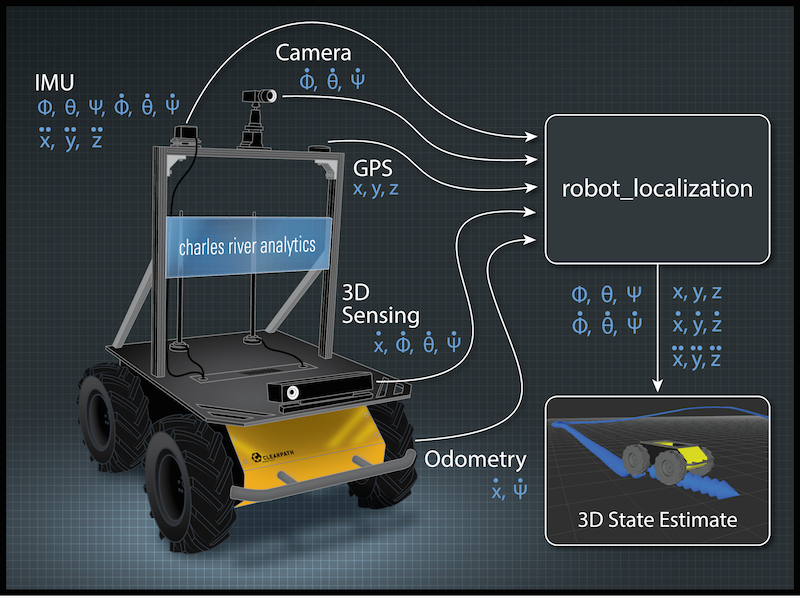
\includegraphics[angle=0,width=0.5\linewidth]{rl}}
\caption[]{Localization Illustration \cite{clearpath}}
\label{fig:robotlocalization}
\end{figure}

Localization is an important step for any autonomous or partially autonomous system hoping to navigate in the physical world. While autonomous driving is not a primary goal for our project, localization is a necessary step for creating an accurate map of the environment. 

ROS provides a framework for developing localization systems and provides several cutting-edge algorithms for fusing sensor data into an accurate position estimate. For our vehicle we are combining the LIDAR, accelerometer, gyroscope, GPS, wheel sensor and camera data using an Extended Kalman filter to generate an accurate position estimate. Using this position estimate, we will then build both 2D and 3D maps of the environment. 

We aim to have our system be able to determine the position of the Rover within 1 meter after traveling 100 meters and generate a map while traveling.

We are using an implementation of an extended kalman filter for state estimation through the ROS robot\_localization package. This package takes input from an arbitarary number of sensors and produces an estimate of the robot's 15 dimensional state, [x,y,z,roll,pitch,yaw,vx,vy,vz,vroll,vpitch,vyaw,ax,ay,az]\cite{Moore2016}. 

The localization of the vehicle is performed in two stages, first taking into account only sensors which produce a continuous estimate of the robot state (ie. Tachometer, IMU) for use in the future autonomous driving and local path planning. The second state takes into account discontinuous sensor data (ie. GPS, SLAM) to produce a more accurate, but sometimes 'jumpy' position estimate. 

Robot state data from many soures are combined in order to create a more accurate estimate of the rover state. The first source is known as the vehicle odometry, combining the tachometer data (forward speed sensor) as well as the steering angle to generate an estimate for the forward velocity of the vehicle as well as the yaw rate (turning rate). In order to get from the steering angle and velocity to the yaw rate estimate, a simple kinematic model of the vehicle is used, leading to the following equation for yaw rate ($\dot{\Psi}$), as a function of forward speed ($\mu_x$), wheel base (L) and steering angle ($\phi_s$).

\begin{equation}
\dot{\Psi} = \frac{\mu_x}{L}\tan{\phi_s}
\end{equation}

The second source of data comes the Inertial Measurement Unit (IMU), which includes 3 sensors; a 3-axis acceleromter, a 3-axis rate gyro and a 3 axis-magnetometer. We chose the CH Robotics UM7 IMU to use on the vehicle because of it's relatively low price point, existing integration with ROS and it's active user base. Most IMU's have filtering on the device and in the case of the UM7, it outputs an orientation estimate (yaw,pitch,roll) as well as the raw sensor data. We chose to incorporate the yaw, pitch and roll estimates in our Kalman filter instead of the raw sensor data. 

Next, the GPS unit, a Novatel Propak-LB, outputs position and velocity estimates in the form of standard NMEA strings. Preexisting ROS nodes enable us to input these strings and incorporate the GPS data into our state estimate. The GPS has the added benefit of performing it's own estimate of the covariance (a statistical measure of the estimate's certainty). The Kalman Filter utilizes the covariance to weigh the GPS more heavily when the GPS has more satellite's in view.

Finally, the rover has 2 lidar sensors available. A statically mounted unit on the front grill and a tilting unit on a gimbal mounted on top of the vehicle. For localization, we are using the unit mounted on the front of the vehicle, along with a ROS package called hector\_slam to produce an estimate for the robot's state. The SLAM (Simultaneous Localization and Mapping) process compares the current laser scan to a map or past data to estimate the movement of the vehicle. The SLAM process also provides us with a 2d map of the environmet which can be saved and used for navigation at a later time..